%|//////////////////////////////////////|\\\\\\\\\\\\\\\\\\\\\\\\\\\\\\\\\\\\\|%
%|//////////////////////////| Objetivo del Proyecto |\\\\\\\\\\\\\\\\\\\\\\\\\|%
%|//////////////////////////////////////|\\\\\\\\\\\\\\\\\\\\\\\\\\\\\\\\\\\\\|%
\section{Objetivo del Proyecto}
% El objetivo es la respuesta a la pregunta “¿para qué?”; tiene que satisfacer alguna necesidad del usuario.

El presente proyecto consiste en el diseño y desarrollo de un sistema de calibración de impedancia y ajuste por electrodeposición (galvanoplastía). Este instrumento se utilizará en el futuro en aplicaciones biomédicas, más precisamente en la fabricación de electrodos de registro extracelular.



%|//////////////////////////////////////|\\\\\\\\\\\\\\\\\\\\\\\\\\\\\\\\\\\\\|%
%|////////////////////////| Descripción del Proyecto |\\\\\\\\\\\\\\\\\\\\\\\\|%
%|//////////////////////////////////////|\\\\\\\\\\\\\\\\\\\\\\\\\\\\\\\\\\\\\|%
\section{Descripción del Proyecto}
% En esta sección se responde la pregunta “¿cómo?”. Aquí se enumeran las prestaciones, las funciones y el comportamiento o uso del equipo.
El equipo consiste en un circuito con un microcontrolador que genera señales senoidales y continuas para medir y corregir las impedancias, respectivamente. Incluye una cuba conductora, que contiene una solución acuosa donde se colocan los electrodos. Éstos son similares a un filamento de cobre recubierto con esmalte aislante en su totalidad, excepto en los extremos, los cuales uno va sumergido en la solución y el otro conectado al equipo por medio de un conector especial.

El sistema funciona con 1, 4, 8, 12 ó 16 electrodos, corrigiendo de a uno por vez. El usuario coloca los electrodos procurando que no se produzcan cortocircuitos entre los mismos (se debería detectar esto antes de comenzar). Hay tres opciones: medir, calibrar y corregir. La primera permite ver el/los valor/es de la/s impedancia/s colocada/s en los conectores. La segunda, calibrar el equipo, tal como su nombre lo indica. La opción de corregir permite que el usuario seleccione la impedancia final deseada, el tiempo máximo de espera para la corrección y dé la orden de inicio. Luego de algunos chequeos básicos se da comienzo al proceso. Al terminar con todos los electrodos, se muestra la impedancia final de cada uno. 

En líneas generales, el sistema consta de módulos de amplificación y filtros de PWM que permiten generar una señal senoidal con el microcontrolador, además de controlar la señal de offset. Asimismo, hay una fuente de corriente controlada por tensión que permite inyectar corriente continua al sistema para poder disminuir las impedancias necesarias por galvanoplastía. 

La señal de salida del PWM es una corriente senoidal de \SI{1}{\kilo\hertz}, con uno de los siguientes valores de amplitud: $\{\SI{30}{\nano\ampere}, \SI{80}{\nano\ampere}, \SI{120}{\nano\ampere}, \SI{200}{\nano\ampere}\}$. Éstos se seleccionan con un multiplexor dependiendo del rango de impedancias: $\{0-\SI{2}{\mega\ohm}, 0-\SI{8}{\mega\ohm}, 0-\SI{20}{\mega\ohm}, 0-\SI{60}{\mega\ohm}\}$. Considerando la ley de Ohm y midiendo el valor pico de tensión, se calcula la impedancia del electrodo en estudio como $Z@\SI{1}{\kilo\hertz} = \frac{\hat{v}}{\hat{\i}}$. Este valor se puede disminuir porque la solución acuosa contiene oro o plata, de modo de que se produce un recubrimiento por galvanoplastía sobre el electrodo y así disminuye la impedancia. Si este proceso es necesario o no, dependerá del resultado previo y de la comparación entre el valor obtenido en la medición y el de referencia establecido previamente por el usuario. Se emplea un multiplexor analógico para ir seleccionando cada electrodo y otro en paralelo con éste, que será eventualmente utilizado para verificar que no haya cortocircuitos entre electrodos. 

Cada \SI{1}{\minute} se mide la impedancia y se corrige de ser necesario. Este proceso se repite tantas veces como se requiera hasta llegar al valor de impedancia deseada determinado previamente en la configuración. Los valores aceptables para empezar el proceso están entre \SI{1}{\mega\ohm} y \SI{8}{\mega\ohm}. Además, hay que pautar un tiempo máximo de sensado y corrección, para que el sistema deje de actuar en caso de haber pasado ese tiempo sin haber llegado al valor buscado. Éste puede valer 10, 20, 30, 40, 50 ó 60 minutos.

%|//////////////////////////////////////|\\\\\\\\\\\\\\\\\\\\\\\\\\\\\\\\\\\\\|%
%|/////////////////////////| Periféricos Principales |\\\\\\\\\\\\\\\\\\\\\\\\|%
%|//////////////////////////////////////|\\\\\\\\\\\\\\\\\\\\\\\\\\\\\\\\\\\\\|%

% Los periféricos son los elementos ajenos al microcontrolador con los que interactúa el equipo y deben estar claramente definidos (por ejemplo: motores, display, teclado, puertos de comunicación, sensores, etc.)

El dispositivo tiene una pantalla LCD donde se muestran las opciones de configuración para seleccionar a través de un menú y también los resultados del proceso, además de los mensajes de error o alerta (en caso de ocurrir algún imprevisto o no llegar al valor deseado en el tiempo pautado, por ejemplo). Las opciones se seleccionan desde un teclado de 4 botones (\texttt{ok}, \texttt{cancelar}, \texttt{mover izquierda}, \texttt{mover derecha}).

Además, como periféricos principales están los circuitos mencionados antes, a través de los cuales se interactúa directamente con los electrodos. Asimismo, otros elementos importantes con los que interactúa el microcontrolador son los multiplexores, que tienen 2 ó 4 entradas de control, según sean de 4 canales o 16, y la cuba electrolítica donde se produce la reacción química para disminuir la impedancia, que está compuesta por un material conductor, el cual también debe conectarse.


%|//////////////////////////////////////|\\\\\\\\\\\\\\\\\\\\\\\\\\\\\\\\\\\\\|%
%|///////////////| Características y Especificaciones Mínimas |\\\\\\\\\\\\\\\|%
%|//////////////////////////////////////|\\\\\\\\\\\\\\\\\\\\\\\\\\\\\\\\\\\\\|%

% Las especificaciones acotan las bondades del equipo. Deben listarse los rangos de funcionamiento o requerimientos externos (por ejemplo: tensión de alimentación, consumo, temperatura de funcionamiento, protocolos de comunicaciones, rangos de medición, etc.)

Las especificaciones del sistema son:

\begin{table}[H]
\begin{center}
\begin{tabular}{|r|l|}
    \hline
    Tensión de alimentación &
    \SI{5}{\volt} \\ \hline
    Rango de impedancias de los electrodos medidos &
    \SI{0}{\mega\ohm} - \SI{60}{\mega\ohm} (@ \SI{1}{\kilo\hertz})\\ \hline
    Impedancia buscada & $\simeq$ \SI{1}{\mega\ohm}\\ \hline
    Cantidad de electrodos a conectar &
    1, 4, 8, 12 ó 16 \\ \hline
    Tiempo máximo de corrección por electrodo &
    \SI{90}{\minute} (*)\\ \hline
    Modo medición & señal senoidal, \SI{1}{\kilo\hertz}, error $<$ 20 \% \\ \hline
    Modo corrección & señal continua 30/80/120/\SI{200}{\nano\ampere}, error $<$ 20\% \\ \hline
\end{tabular}
\end{center}
\end{table}

(*) una vez cumplido este tiempo se abandonan los esfuerzos.



%|//////////////////////////////////////|\\\\\\\\\\\\\\\\\\\\\\\\\\\\\\\\\\\\\|%
%|/////////////////////| Diagrama en Bloques (hardware) |\\\\\\\\\\\\\\\\\\\\\|%
%|//////////////////////////////////////|\\\\\\\\\\\\\\\\\\\\\\\\\\\\\\\\\\\\\|%
\pagebreak
\section{Diagrama en Bloques (hardware)}
% El esquema general de interconexión de todos los dispositivos importantes se representa mediante un diagrama en bloques.
El diagrama de bloques aquí abajo muestra la interconexión de los dispositivos más relevantes del sistema.
\begin{center}
    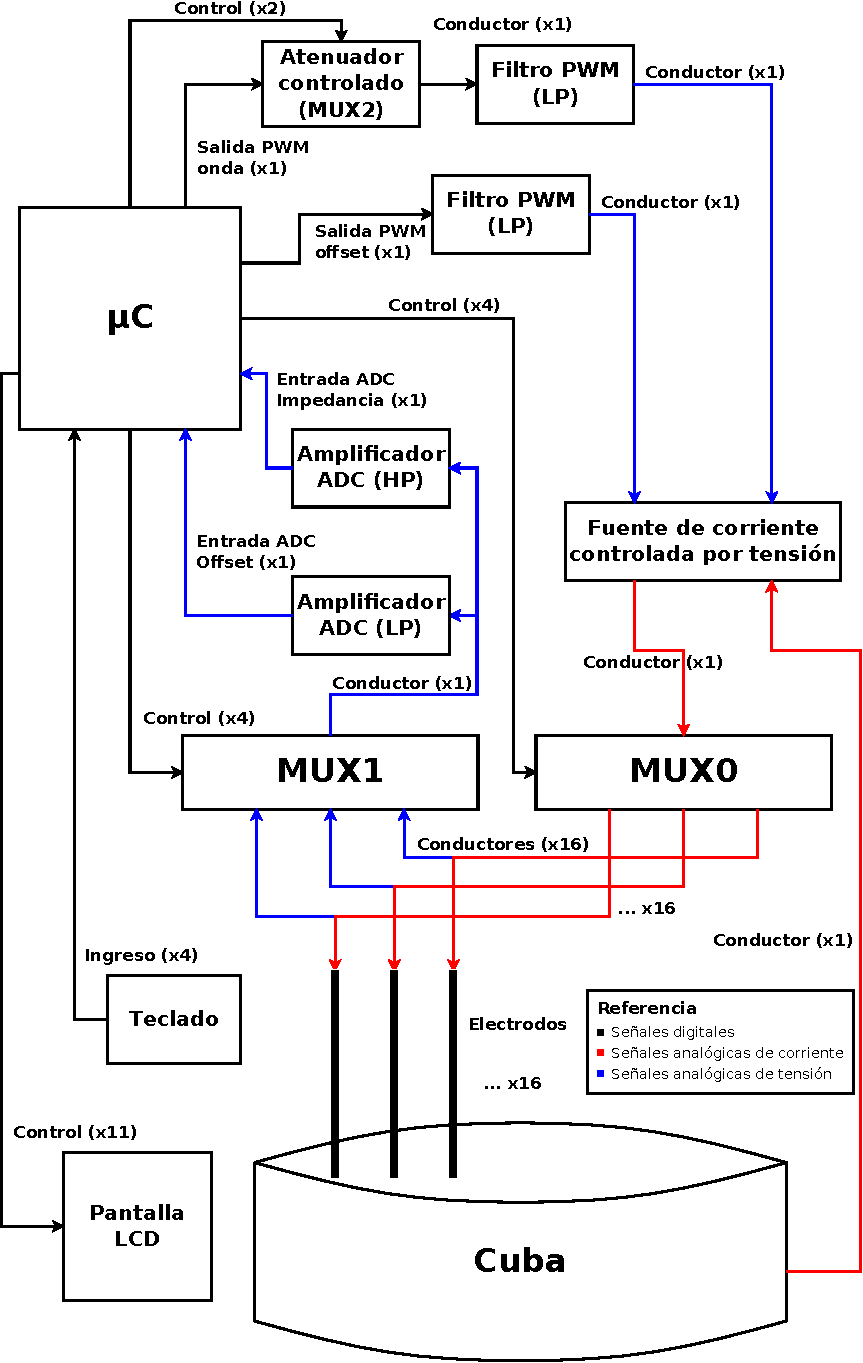
\includegraphics[scale=0.9]{bloques}
\end{center}



%|//////////////////////////////////////|\\\\\\\\\\\\\\\\\\\\\\\\\\\\\\\\\\\\\|%
%|//////////////////////| Diagrama de Flujo (firmware) |\\\\\\\\\\\\\\\\\\\\\\|%
%|//////////////////////////////////////|\\\\\\\\\\\\\\\\\\\\\\\\\\\\\\\\\\\\\|%
\section{Diagrama de Flujo  (firmware)}
% El diagrama de flujo ilustra de manera general la interacción entre los distintos bloques (o rutinas) de código.
El diagrama de flujo final del proyecto es el siguiente:
\begin{center}
    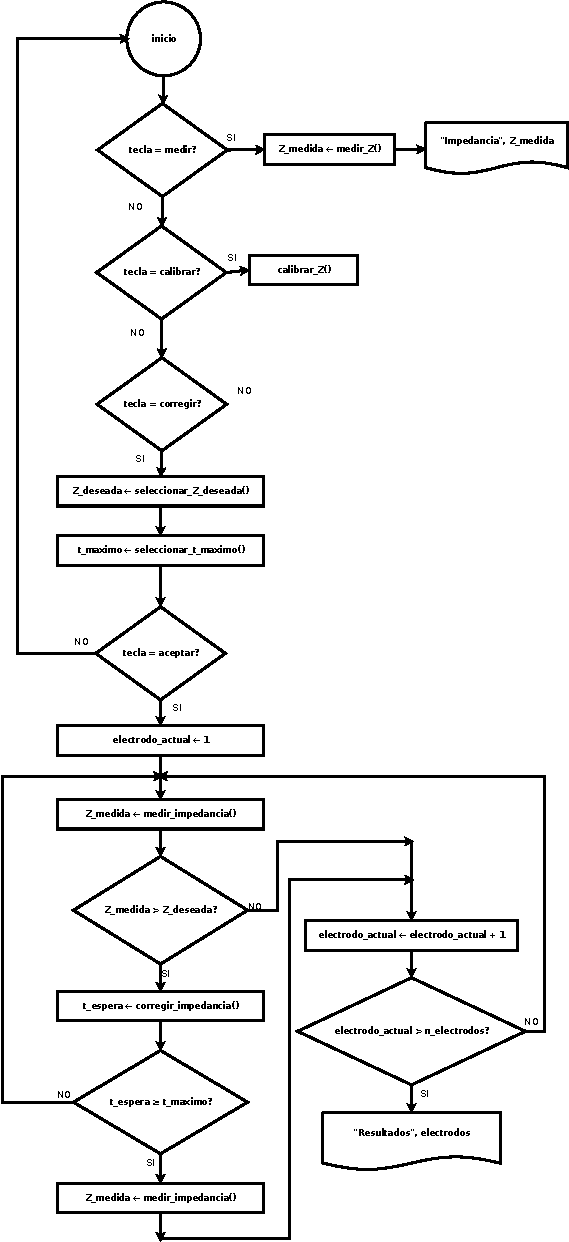
\includegraphics[scale=1]{flujo}
\end{center}



%|//////////////////////////////////////|\\\\\\\\\\\\\\\\\\\\\\\\\\\\\\\\\\\\\|%
%|//////////////////////////| Circuito Esquemático |\\\\\\\\\\\\\\\\\\\\\\\\\\|%
%|//////////////////////////////////////|\\\\\\\\\\\\\\\\\\\\\\\\\\\\\\\\\\\\\|%
\section{Circuito Esquemático}
% La representación del circuito eléctrico final del prototipo debe realizarse en algún sistema CAD; no es necesario el diseño del circuito impreso (PCB), basta con el circuito esquemático.
A continuación se muestra el circuito esquemático correspondiente al prototipo, así como también el diseño del PCB. Ambos fueron realizados con el programa KiCad.\\
 
\hspace{-1.8cm}
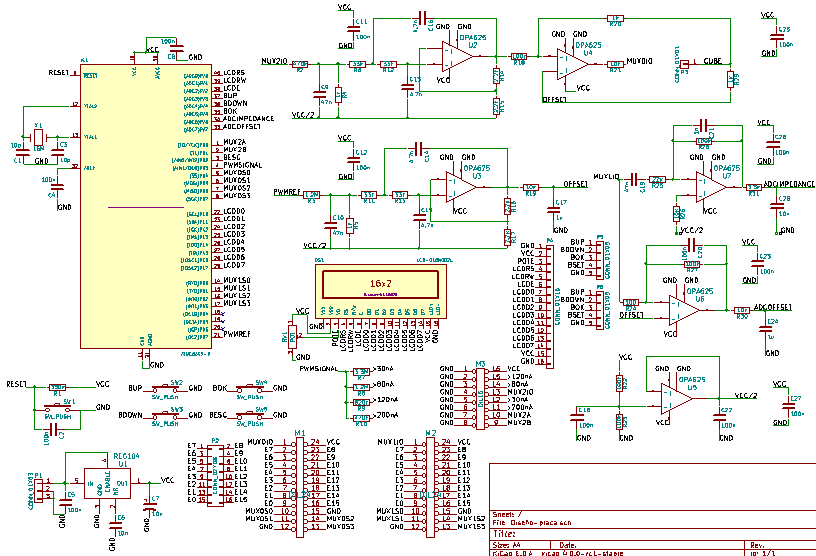
\includegraphics[scale=0.7]{circuito_esquematico}

\hspace{-1cm}
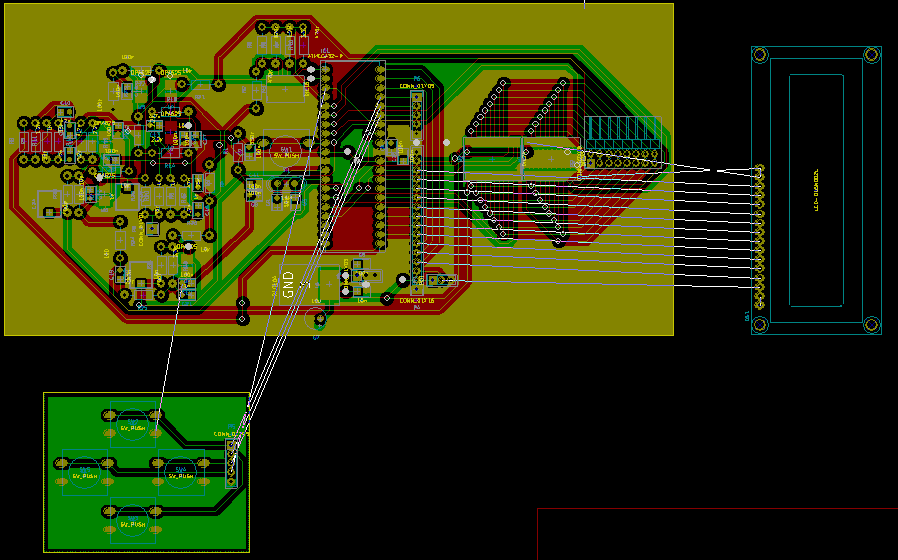
\includegraphics[scale=0.9]{circuito_PCB}


%|//////////////////////////////////////|\\\\\\\\\\\\\\\\\\\\\\\\\\\\\\\\\\\\\|%
%|////////////////| Listado de Componentes y Costos Estimados |\\\\\\\\\\\\\\\|%
%|//////////////////////////////////////|\\\\\\\\\\\\\\\\\\\\\\\\\\\\\\\\\\\\\|%
\pagebreak
\section{Listado de Componentes y Costos}
% En esta sección se debe incluir el listado final de componentes con sus respectivos costos. Además deben incorporar la estimación de horas-hombre insumidas en la realización del proyecto. 
Los componentes que se emplearon para la construcción del dispositivo se muestran en la tabla siguiente:

\begin{table}[H]
\begin{center}
\begin{tabular}{|l|rr|}
    \hline
    \textbf{Componente} & \multicolumn{2}{c|}{\textbf{Costo}} \\ \hline
    Atmega32            & \hspace{2.8cm}\$ &   164.5 \\ \hline
    OPA625 x6 (*)       & \$               &   166.2 \\ \hline
    REG104 (*)          & \$               &   70.0 \\ \hline
    CD74HC4067 x2 (*)   & \$               &   16.8 \\ \hline
    SN74LV4052 (*)      & \$               &   5.0 \\ \hline
    Resistencias x30    & \$               &   9.6 \\ \hline
    Potenciómetro       & \$               &   6.7 \\ \hline
    Capacitores x31     & \$               &   43.1 \\ \hline
    Display LCD         & \$               &   120.0 \\ \hline
    Pulsadores x5       & \$               &   18.8 \\ \hline
    Cristal 16 Mhz      & \$               &   6.0 \\ \hline 
    Conectores          & \$               &   8.6 \\ \hline       
    Placa Epoxy         & \$               &   120.0 \\ \hline
    Zócalo              & \$               &   3.0 \\ \hline
    Jack power          & \$               &   3.2 \\ \hline           
    TOTAL               & \$               &   761.5 \\ \hline
\end{tabular}
\end{center}
\end{table}

Los componentes marcados con un asterisco(*) son de Texas Instruments y en el marco del IIBM y de la Facultad se obtuvieron como muestras gratis. Por ende, para este trabajo en particular el costo de los componentes utilizados fue de $\$ 503.5$.\\

En cuanto a las horas-hombre involucradas, se puede estimar un número de 300 horas/hombre. 



%|//////////////////////////////////////|\\\\\\\\\\\\\\\\\\\\\\\\\\\\\\\\\\\\\|%
%|///////////////////////////////| Resultados |\\\\\\\\\\\\\\\\\\\\\\\\\\\\\\\|%
%|//////////////////////////////////////|\\\\\\\\\\\\\\\\\\\\\\\\\\\\\\\\\\\\\|%
\section{Resultados}
% No siempre se logran los objetivos propuestos (o al menos en su totalidad); es importante que puedan validar y/o ajustar las expectativas indicando las limitaciones finales del prototipo construido.

Debido a las complicaciones en el diseño del hardware y los reiterados cambios que fueron hechos con el desarrollo del proyecto, se modificó el circuito de manera de poder medir impedancias del orden de los $k\Omega$, en vez de $M\Omega$, ya que las señales eran muy pequeñas y no se diferenciaban de las señales de ruido. Los nuevos rangos de medición son: $\{0-\SI{143}{\kilo\ohm}, \SI{143}{\kilo\ohm}-\SI{243}{\kilo\ohm}, \SI{243}{\kilo\ohm}-\SI{335}{\mega\ohm}, \SI{335}{\kilo\ohm}-\SI{900}{\mega\ohm}\}$.
 
Con estas modificaciones se pudo obtener un funcionamiento acorde a lo esperado, visualizando valores de impedancia en el display con un error aproximado del 15\%. Este error se debe a la alinealidad que genera el circuito. Como hipótesis, es posible considerar que se debe a que la fuente de corriente ya no se comporta linealmente con estos nuevos valores de corriente (se aumentaron 100 veces). 

Fue posible observar el correcto funcionamiento de las rutinas de impresión por display, conversión ADC, obtención de la mediana a través de ordenamiento de tablas por burbujeo, utilización de pulsadores externos, timers, interrupciones, PWM. Se pudo observar, con el uso de un osciloscopio, el funcionamiento de la rutina de corrección de electrodos, observando un valor de continua. En la imagen a continuación se puede ver cómo en una primera etapa no hay corriente circulando, luego se observa la senoidal que sirve para medir y finalmente un valor de continua que permite corregir el valor de la impedancia. 

\hspace{-1cm}
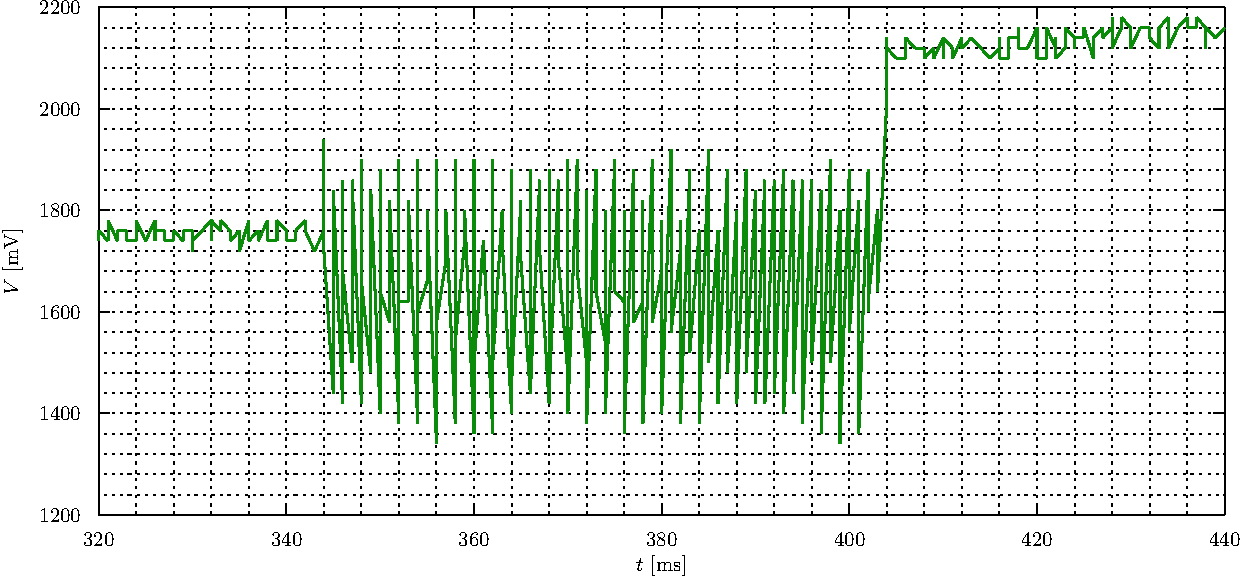
\includegraphics[scale=0.85]{osciloscopio}

%|//////////////////////////////////////|\\\\\\\\\\\\\\\\\\\\\\\\\\\\\\\\\\\\\|%
%|//////////////////////////////| Conclusiones |\\\\\\\\\\\\\\\\\\\\\\\\\\\\\\|%
%|//////////////////////////////////////|\\\\\\\\\\\\\\\\\\\\\\\\\\\\\\\\\\\\\|%
\section{Conclusiones}
% En este punto tienen que describir mejoras posibles que podrían hacerse al equipo, cambios sugeridos en función de las experiencias aprendidas  y cualquier otra sugerencia relacionada con el proyecto.
Como mejoras, se puede mencionar que es altamente recomendable contar con una opción más en el menú para determinar si dos electrodos están o no en cortocircuito. Para ello, se emplea el segundo multiplexor (que aparece en el diseño pero no forma parte de este proyecto). Se podría realizar inyectando señal en cada electrodo y chequeando sobre cada uno de los restantes que no se reciba un nivel elevado de ésta. Además, agre

Por otro lado, sería útil para el usuario que hubiera alguna identificación para ver cuándo mide correctamente cada electrodo, si hay dos en cortocircuito y demás cuestiones que momentáneamente sólo aparecen al final del proceso (leds, por pantalla, etc), así el usuario no tiene que esperar hasta el final para ver si funcionó correctamente o no. 


%|//////////////////////////////////////|\\\\\\\\\\\\\\\\\\\\\\\\\\\\\\\\\\\\\|%
%|////////////////////////////////| Apéndices |\\\\\\\\\\\\\\\\\\\\\\\\\\\\\\\|%
%|//////////////////////////////////////|\\\\\\\\\\\\\\\\\\\\\\\\\\\\\\\\\\\\\|%
\section{Apéndices}
% Como complemento al informe, en esta sección deben agregar el listado completo de software, las hojas de datos principales y cualquier otra información, referencia o cálculo relacionada con el proyecto (por ejemplo el uso de interrupciones).

\subsection{Cálculos}
A continuación se muestran los cálculos involucrados en la obtención de los parámetros $p$ por el que habrá que multiplicar a la medición del valor pico para obtener la impedancia. Vale aclarar que estos son valores iniciales y luego serán corregidos durante la calibración automática del equipo.

\hspace{-1cm}
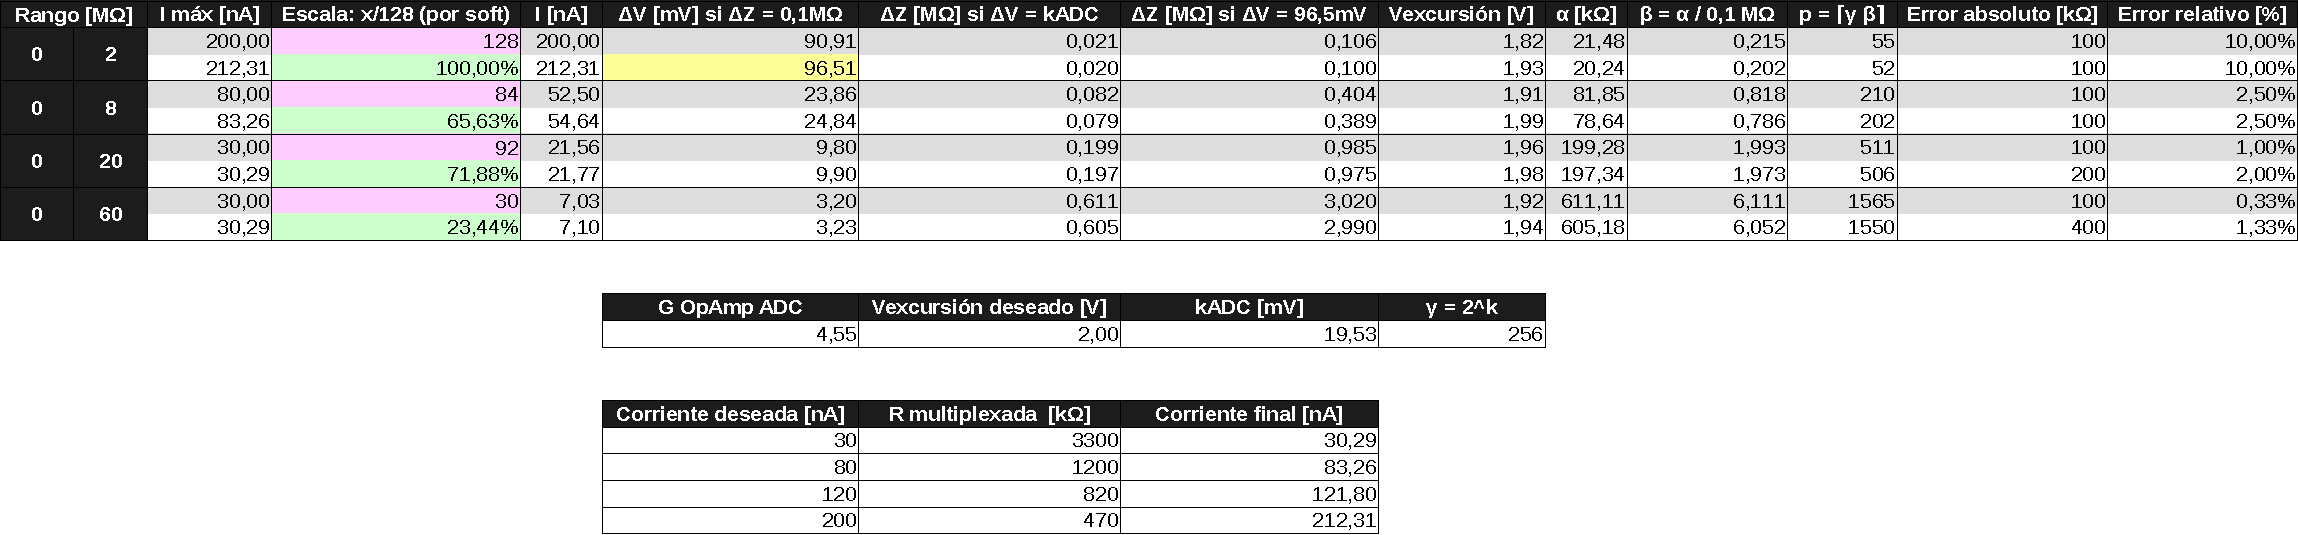
\includegraphics[scale=0.5]{calculos}

\subsection{Hojas de datos}

Los componentes empleados son:
\begin{table}[H]
\begin{center}
\begin{tabular}{|l|c|}
    \hline
    \textbf{Componente} & \textbf{Hoja de datos} \\ \hline
    Atmega32      & \url{http://www.atmel.com/images/doc2503.pdf} \\ \hline
    OPA625        & \url{http://www.ti.com/lit/ds/symlink/opa625.pdf} \\ \hline
    REG104        & \url{http://www.ti.com/lit/ds/symlink/reg104.pdf} \\ \hline
    CD74HC4067    & \url{http://www.ti.com/lit/ds/symlink/cd74hc4067.pdf} \\ \hline
    SN74LV4052    & \url{http://www.ti.com/lit/ds/symlink/sn74lv4052a.pdf} \\ \hline
    Display LCD   & \url{http://elmicro.com/files/lcd/gdm1602a\_datasheet.pdf} \\ \hline        
\end{tabular}
\end{center}
\end{table}


\subsection{Códigos fuente}
En las siguientes páginas se incluyen a modo de apéndice todos los archivos que conforman el firmware de equipo.
